\documentclass[10pt]{article}

\usepackage{amsmath}
\usepackage{graphicx}
\usepackage[margin=0.7in]{geometry}
\usepackage{float}
\usepackage{listings}
\usepackage[utf8]{inputenc}
\usepackage[parfill]{parskip}  
\usepackage{multicol}
\usepackage{siunitx}
\usepackage[dvipsnames]{xcolor}
% \usepackage{hyperref}
\usepackage{cleveref}
\usepackage{cite}
\usepackage{caption}
\usepackage{tabularx}
%\usepackage{mathabx}
\usepackage{titling}

\captionsetup{width=0.6\linewidth}

\newcommand{\rhomax}{\rho_{\text{max}}}
\newcommand{\relerr}{\epsilon_{\text{rel}}}
\newcommand{\bigO}[1]{\mathcal{O}(#1)}

\graphicspath{{../results/}}

\newcommand\myshade{50}
\colorlet{mylinkcolor}{violet}
\colorlet{mycitecolor}{YellowOrange}
\colorlet{myurlcolor}{Aquamarine}

% \hypersetup{
%   linkcolor  = mylinkcolor!\myshade!black,
%   citecolor  = mycitecolor!\myshade!black,
%   urlcolor   = myurlcolor!\myshade!black,
%   colorlinks = true,
% }

% \pretitle{%
%     \begin{center}
%     \LARGE
%     }
% \posttitle{\end{center}}


\begin{document}
\title{The Solar System
\\ Project 3
\\ FYS3150}
\author{Ragnar Bruvoll \and Halvard Sutterud}
%\author{Halvard Sutterud}
\date{October 2017}
\maketitle{\begin{center}\end{center}}
\pagenumbering{gobble}
\thispagestyle{empty}

\begin{figure}[H]
    \centering
    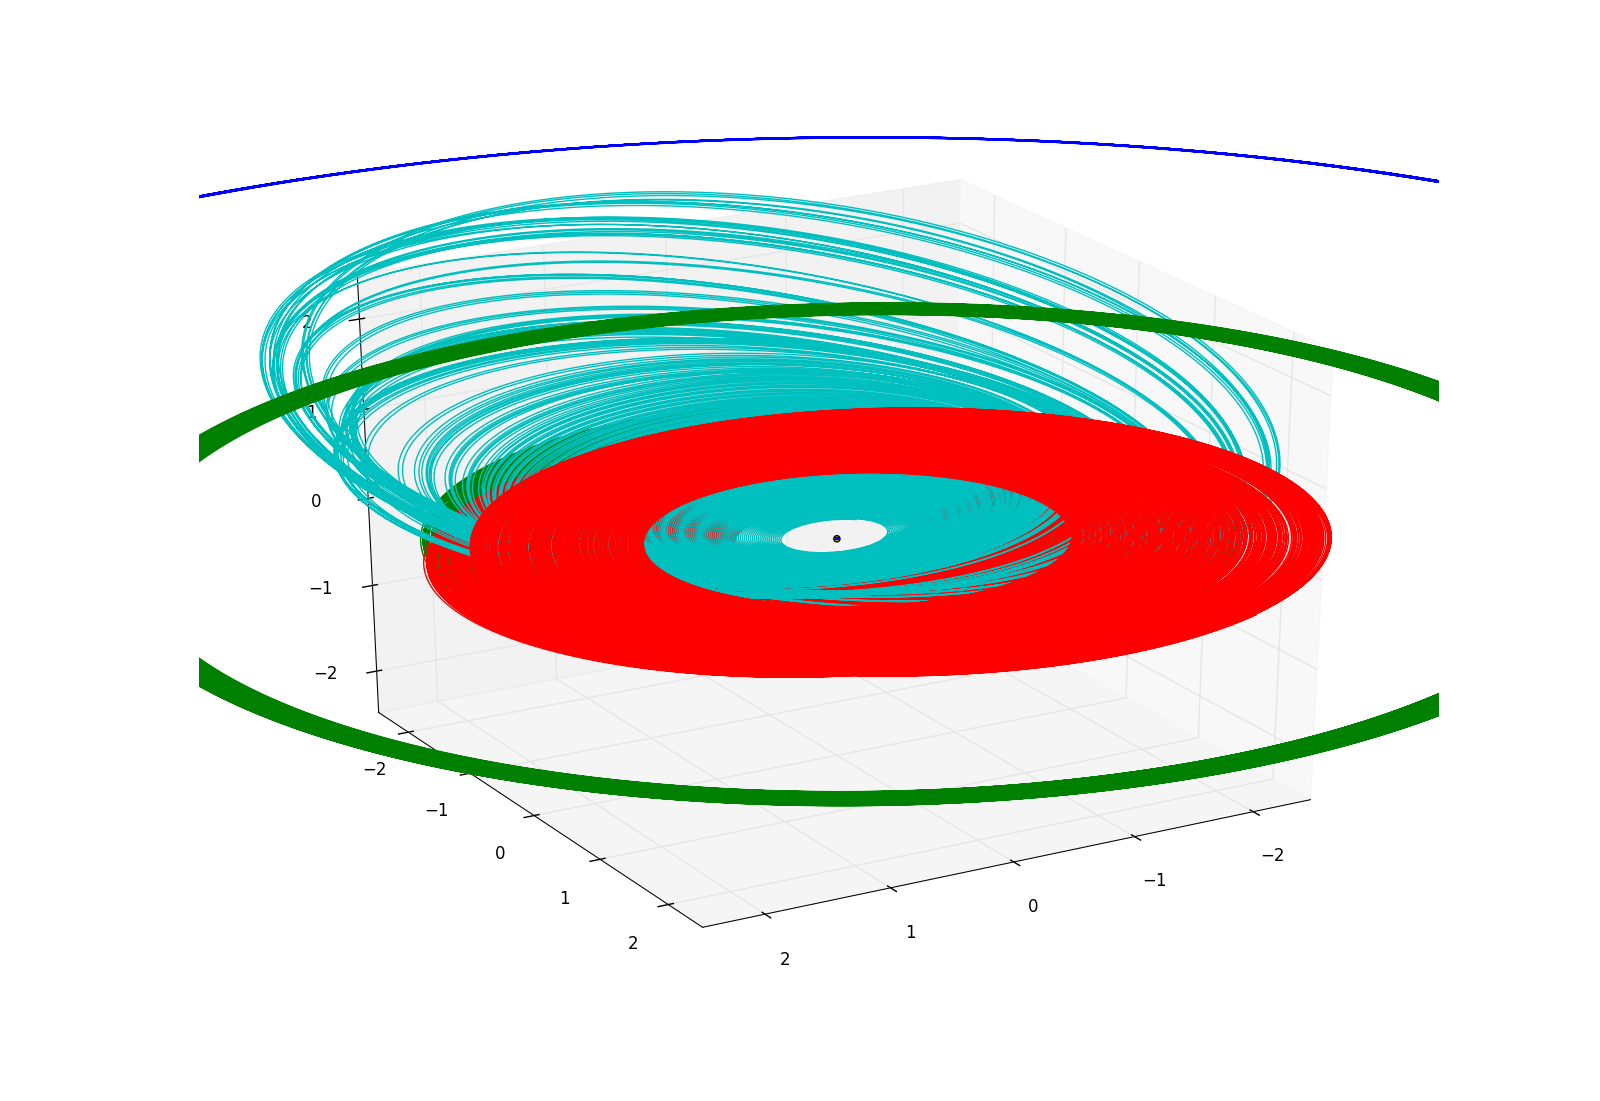
\includegraphics[width=0.8\linewidth]{../results/front.png}
    \label{fig:name}
\end{figure}

\begin{abstract}
    We study a model of the solar system as gravitationally interacting
    celestial bodies.  Using an object oriented approach, we implement
    classes in \texttt{c++} to solve the differential equations of the
    mechanics of the solar system in \texttt{c++}. We compare the effectiveness of
    two methods for numerical differentiation, namely Forward Euler and
    Velocity Verlet, and discuss their stabilities in terms of energy
    conservation. Some properties of the solar system are studied, including
    escape velocity for a planet in a two body system, a modified three
    body problem, and finally the phase precession of a Sun-Mercury system
    with relativistic corrections. 
    The Forward Euler integration method is found to be less costly per
    iteration, but unlike the verlet method it doesn't conserve energy and
    is unstable over longer time periods (as seen in the front figure) . 
\end{abstract}

\newpage



\begin{multicols}{2}
\tableofcontents

% \newpage
\pagenumbering{arabic}

\section{Introduction}
The purpose of this project is to solve the differential equations of the
mechanics of the solar system in an efficient way with precise results.
There are several different algorithms to calculate the objects orbiting a
star, each with their strengths and weaknesses. A couple of these will be
showcased and compared to examine which one is preferable in our case.

Our entire simulation is based on Newton's second law of montion
\begin{equation}
    F_G = \frac{M_\Sun M_{Earth}}{r^2}
\end{equation}
which turns out to be an adequate estimation for most objects in
regular solar systems. In order to create a simulation with a desirable
precission, a large number of iterations is necessary. The solar system is
a complex one, with many factors and interactions. So our biggest challenge
is to efficiently manipulate our computer with a program that exploits all
its processing power without taking too much of our time. In other words,
we want to make an as simple program as possible, without losing any of its
precission. Different tricks and methods for simplifying the algorithm will
therefore be explained and implemented. 

We will gradually complicate our system in order to make it more realistic,
and finally include a correction from of general relativity on objects
significantly affected by it, where we prevously only used newtonian
physics.

%%%%%%%%%%%%%%%%%%%%%%%%%%%%%%%%%%%%%%%%%%%%%%%%%%%%%%%%%%%%%%%%%%%%%%%%%%%
\section{Theory}
\subsection{Units}
 % \subsection{Discretizing equations and defining acceleration}
Using Newton's second law, which states that the sum of all the forces
equals mass times acceleration, $\sum F=ma$, we can calculate the
acceleration of the planet in relation to the Sun. Assuming circular
orbits, we know this acceleration to be the sentripetal acceleration, and
the force is the gravitational force

\begin{equation}
    F_G = M_\Earth a = M_\Earth\frac{v^2}{r} = G\frac{M_\Sun M_\Earth}{r^2}
\end{equation}



with the earth as an example. We will be using the astronomical symbols for
the celestial bodies; $M_\Earth$ is then the mass of the Earth and $M_\Sun$
the mass of the sun. With this in mind, we can simplify the equations and
calculations by using astronomical units and years as unit lengths. So
instead of using $r = 1.5\cdot10^{11}m$ and , we'll simply assert $r =
1AU$. With simple multiplication, the expressions for sentripetal force and
gravitational force can be written as 

\begin{equation}\label{eq:circVel}
    \Rightarrow v^2r = GM_\Sun
\end{equation}

and with the new unit lengths applied we can simplify it further. We know
that the radius from the earth to it's spin system's centre is one
astronomical unit, 1 AU. The orbit speed is one round per year, that is
2$\pi$AU/year. This means

\begin{equation}
    GM_\Sun = v^2r = 4\pi^2AU^3/year^2
\end{equation}

We can now substitute this constant and get an expression for the general
acceleration of any object with an circular orbit around the Sun

\begin{equation}
    M_\Earth a = GM_\Sun\frac{M_\Earth}{r^2}
\end{equation}

\begin{equation}
    a = \frac{4\pi^2}{r^2}
\end{equation}
with the acceleration in units $[a] = \SI{}{AU/yr^2}$. 

The unit of energy is also redefined, with new units for mass, length and time:
\begin{align}
    E &= mass\cdot\frac{length^2}{time^2} = M_\texorpdfstring{\Sun}{}\frac{AU^2}{year^2}\nonumber\\ 
    &= 1.989\cdot10^{30}kg\frac{(1.4959\cdot10^{11}m)^2}{(60\cdot60\cdot24\cdot365s)^2}\nonumber\\
    &\equiv J_\Sun,
\end{align}

where we introduced a new energy unit, the Astrojoule $J_\Sun \approx 4.5\cdot10^{37}J  $.  Please note
that these are the universal units for all equations and figures in this
report.

% \subsection{Bound orbits}
% We know from Keplers laws that planetary motion takes the form of cone
% sections. Except for a practically infeasible perfect circular orbit, 
% an orbiting body follows the trajectory of an ellipse. The energy of these
% We also know that the 

\subsection{Energy calculation}
As all the forces involved are conservative, the energy of the system
should be conserved. If this is not the case, it could be an indication
that out program is not stable. For stability analysis, we will therefore
make sure that the sum of the systems energies is constant. The energies
are given by the following equations 

\begin{align}\label{eq:energies}
    T &= \sum_{i=1}^N \frac{1}{2}mv_i^2 & V &= \sum_{i=1}^N \sum_{j=i+1}^N
    -r_{i,j}|F_{i,j}|
\end{align}

where $T$ is the total kinetic energy, found by summing over the kinetic
energies of all $N$ objects, and $V$ is the potential energies due to
gravitational force between bodies $F_{i,j}$, given by

\begin{equation}
    F_{i,j} =  G\frac{M_iM_j}{r_{i,j}^2}
\end{equation}

with $M_i$ being the mass of object $i$ and $r_{i,j} = |\vec r_i - \vec
r_j|$ as the distance between two objects.

\subsubsection{Escape velocity}
The escape velocity of an object in orbit is achieved when the kinetic energy equals the potential, in this case the gravitational potential;
\begin{align}
    \frac{1}{2}M_\Earth v_e^2 &= GM_\Sun\frac{M_\Earth}{r}\nonumber\\
    v_e &= \sqrt{ \frac{GM_\Sun }{r} }
\end{align}


\subsubsection{Conservation of Angular Momentum}



\subsection{Integration}
As the trajectories of all the objects in the solar system is being
affected by all the other objects at all times, it is quite obvious that
the acceleration is not constant as they would be in a circular orbit. We
therefore need to integrate their position from Newton's equations for each
time step. This can be done with different methods, in our case Euler's
forward algorithm and velocity Verlet method. They're both derived from the
Taylor series. As we cannot make the time steps of the integration
infinitesimaly small, the methods are bound to be incorrect to a certain
degree. The impact of this error will be scrutinized in a later section.

\subsubsection{Taylor expantion}
The Taylor series is an infinite sum of terms given by the function's
derivative at each point. The series is used to express an unknown
curve and it converges closer to the correct value with each degree. 

\begin{equation}
   f(x) =  \sum_{n=0}^\infty\frac{f^{(n)}(a)}{n!}(x-a)^n
\end{equation}

\begin{equation}
    f(x) = f(a)+ \frac{f'(a)}{1!}(x-a)^1+\frac{f''(a)}{2!}(x-a)^2+\cdots
\end{equation}

It is however impossible to add an infinite number of terms, and each term
will further burden the calculating system. But as the value of the terms
decrease for each degree, we can justifiably simplify the series to one of
three terms. This will entail a certain degree of error, but as we will see
it varies between methods, and is often so small we can ignore it.

\subsubsection{Euler's forward algorithm}
The Euler forward method is a first order method, meaning that the local
error is proportional to the step size squared. This incentivizes ut to
pick a step size as small as possible without making the program too slow.
For this method we only use two of the taylor terms, knowing velocity
derived to be acceleration.  

\begin{equation}
    v_{i+1} = v_i +ah
\end{equation}

As for the position, we use the current velocity in the second term to
increase the accuracy.

\begin{equation}
    x_{i+1} = x_i +v_{i}h
\end{equation}

With this algorithm we can calculate the position of the object at as many
point as we like, with an increased error with bigger time steps. The
algorithm requires an initial velocity, position and the acceleration at
each point of the position, which we will derive from the forces action
upon on the object. The Euler method has four FLOPS per time step.\\

This method is good for finding an approximated trajectory, but as we will
see, it is far from perfect.


\subsubsection{Velocity Verlet method}
A more accurate method for finding the trajectory, the velocity and
position that is, would be the velocity Verlet method. This too is based on
the Taylor series, with every term from the fourth and on assumed to be
negligible.

\begin{equation}
    v_{i+1} = v_i +hv_i^{(1)}+\frac{h^2}{2}v_i^{(2)}+O(h^3)
\end{equation}

\begin{equation}
    x_{i+1} = x_i +hx_i^{(1)}+\frac{h^2}{2}x_i^{(2)}+O(h^3)
\end{equation}

where $v_i^{(1)}$ is still the acceleration defined by the acting forces.
We can remove second derivative by substituting it with the first
derivative multiplied with the time step. 

\begin{equation}
    hv_i^{(2)} \approx v_{i+1}^{(1)}-v_i^{(1)}\nonumber
\end{equation}
This applied to our Taylor series gives us
\begin{align}
    v_{i+1} &= v_i + hv_i^{(1)}+\frac{h}{2}\left(v_{i+1}^{(1)}-v_i^{(1)}\right)\nonumber\\
    &= v_i+\frac{h}{2}\left(v_{i+1}^{(1)}+v_i^{(1)}\right)
\end{align}

As for our position calculation, we will use the definition of motion
derivatives, namely $v_i^{(1)}=x_i$.

\begin{align}
    x_{i+1} &= x_i +hx_i^{(1)}+\frac{h^2}{2}x_i^{2}+O(h^3)\nonumber\\
    &= x_i + hv_i + \frac{h^2}{2}v_i^{(1)}
\end{align}

As shown in figure \cref{fig:XXX} this method makes for a more precise
calculation of the trajectories. But with 9 FLOPS per time step, this
method is way more demanding in terms of computational calculation than the
aforementioned.

% \begin{figure}[H]
%     \centering
%     % \includegraphics[width=0.8\linewidth]{XXX.pdf}
%     \caption{XXX}
%     \label{fig:XXX}
% \end{figure}

\subsection{Relativistic corrections}
General relativity predicts corrections to the Newtonian force an object
experiences in the vicinity of a massive object. For Mercury, the
gravitational force is better approximated with the expression

\begin{equation}
    F_G = \frac{GM_{\Sun}M_{\Mercury}}{r^2}
    \left[1+\frac{3l^2}{r^2 c^2}\right] ,
\end{equation}

where  $M_\Sun$ is the mass of the Sun, $M_\Mercury$ is the
mass of Mercury, $l$ is the angular momentum of mercury around the sun
center of mass and $c$ is the speed of light in vacuum. 

\subsection{FLOPS}
FLOPS are floating point operations, meaning the effect of an operator on
an expression. Examples are addition, multiplications etc. Every one of
these operations will consume some processing power. Minimizing the total
number of FLOPS is therefore essential in order to avoid a tedious program.
By counting FLOPS we can attain an implication as to how much time the
operations will consume.
\subsubsection{Euler:} 
\begin{equation}
    \boxed{v_{i+1}=v_i+ah}\ \ , \ \ \boxed{x_{i+1}=x_i+v_ih} 
\end{equation}
With one iteration, that is one time step, the Euler method has 4 FLOPS.

\subsubsection{Verlet:}
\begin{align}
    &\boxed{v_{i+1}=v_i+\frac{h}{2}\left(v_{i+1}^{(1)}+v_{i}^{(1)}\right)}\nonumber\\
    &\boxed{x_{i+1}=x_i+hv_i + \frac{h_2}{2} v_{i}^{(1)}}
\end{align}
By stating a new parameter $h_2 = h^2$ and calculating it before the loop,
we will save one FLOP per iteration. This might not seem significant, but
if the program runs 10 years with 10.000 iterations per year, every FLOP
counts. This tallies up to a total of 8 FLOPS.

In conclusion, the Verlet method is slower than Euler's. 




%%%%%%%%%%%%%%%%%%%%%%%%%%%%%%%%%%%%%%%%%%%%%%%%%%%%%%%%%%%%%%%%%%%%%%%%%%%
\section{Methods}

\subsection{An object oriented approach}
We implement three different classes in
\texttt{c++}; \texttt{CelestialBodies} represents the individual bodies as
point particles, storing their physical variables. These are then stored in
\texttt{SolarSystem}, which represents the environment and the physical
laws. Finally, \texttt{Integrator} is responsible for propagating the
system forward in time, using the forces and an numerical integration
method to find the object positions in the next time step.

The basis of this structure was laid by Anders Hafreager
https://github.com/andeplane/solar-system, providing a basic
forward euler and declaration of many of the member variables and functions
needed for the project. 


\subsection{Two-body problem \texorpdfstring{$\Sun\Earth$}{}} 
We assume a circular orbit of the earth around the sun, and also that the
acceleration of the sun due to the earth is negligible. The
Sun-Earth-system is then initialized by setting the Sun to a fixed position
at $\vec r_\Sun = 0$, and the position of Earth to $\vec r_\Earth =
\SI{1}{AU}\hat e_x$  with velocity $\vec v_\Earth = \SI{2\pi}{AU/yr}\hat e_y$.

The solution of the orbit of Earth is found using both Forward Euler and
Velocity Verlet. 

\subsection{}

\subsection{Stability analysis}
Now that we have established a simple solar system with two bodies, we can
test the stability of our algorithm. We do this by testing different time
steps $\Delta t$. This is applied to both our Euler and our Verlet
algorithm with time steps in $N \in \{5 \to 5 \times 2^{19}\}$ steps per year,
increasing with steps of power of two.

\subsection{Escape velocity}
To study the conditions for a planet to be in a bound state (elliptical orbit), we plot a series of different initial velocities and integrating the force. Then we can observe on the plots what velocity is needed for the earth to leave the orbit. When this velocity is found, we can compare it to the analytical expression, given by expression (10). 

\subsection{Adding Jupiter \texorpdfstring{$\Sun\Earth\Jupiter$}{}}

We analyse the stability of the solar system when including Jupiter
($\Jupiter$) in our previous setup. The initial position of Jupiter is set to
$\vec r_\Jupiter = -\SI{5.2}{AU}\hat e_x$, with velocity $\vec v_\Jupiter =
-\SI{1}{AU/yr}\hat e_y$, found from inserting numbers in \cref{eq:circVel}.
The mass of Earth is now relevant, as we will be calculating the
gravitational effects from all bodies on all the others except on the Sun.
The masses of the objects are listed in the appendix.

\subsubsection{Massive Jupiter }
We then increase the mass of Jupiter to study the effects on the stability
of the orbit of earth. The mass is increased to $10x$ and $1000x$ the
original mass of Jupiter, but otherwise we use the same initial conditions.

\subsubsection{Three-body problem} 
Moving towards a more realistic model of the solar system, we let the Sun
be affected by the gravitational effects of the planets. The initial
conditions are now set from real data. NASA 
has an interface (\texttt{https://ssd.jpl.nasa.gov/horizons.cgi}) to
celestial body initial conditions, which can be parsed by the preprocessor
script \texttt{analyse/read\_horizon.py} (Ephemeris type needs to be set to
VECTORS).  Consider that the velocities received by NASA are assumed to be
around a common barycenter for the whole solar system; if one then excludes
some planets, the total momentum will not be zero and the system will
drift.  
Correcting for this is done with the \texttt{--fix\_barycenter} argument of
\texttt{read\_horizon.py}. It finds the total velocity of the barycenter
and sets it to zero.


\subsection{N-body problem \texorpdfstring{$\Sun\Mercury\Pluto\Earth\Mars\Jupiter\Saturn\Neptune\Uranus\Pluto$}{}} 
Our system now includes several objects that all interact with one another.
We have made sure that our time step is a reasonable one and that the
energy is conserved. The next step is adding all the other planets. We use
the same strategy as with Jupiter, with the relevant data aquired from
NASA. 

\subsection{Mercury perihelion precession \texorpdfstring{$\Sun\Mercury$}{}} 
The final addition to our solar system is applying the non-newtonian
general relativistic effects the sun has on Mercury, with equation (19)

\subsection{Testing and algorithm analysis}
\subsubsection{Stability of \texorpdfstring{$\Delta t$}{}}
\subsubsection{Energy and angular momentum conservation}
\subsubsection{FLOPS}

%%%%%%%%%%%%%%%%%%%%%%%%%%%%%%%%%%%%%%%%%%%%%%%%%%%%%%%%%%%%%%%%%%%%%%%%%%%
\section{Results}
\subsection{Two body problem}
\subsubsection{Stability of $\Delta t$}
As shown in \cref{fig:stab_euler} below, the stability of the algorithm
clearly depends on the size of the time step. The plots shows how the
distance of the planet gradually increases in time.  

\begin{figure}[H]
    \centering
    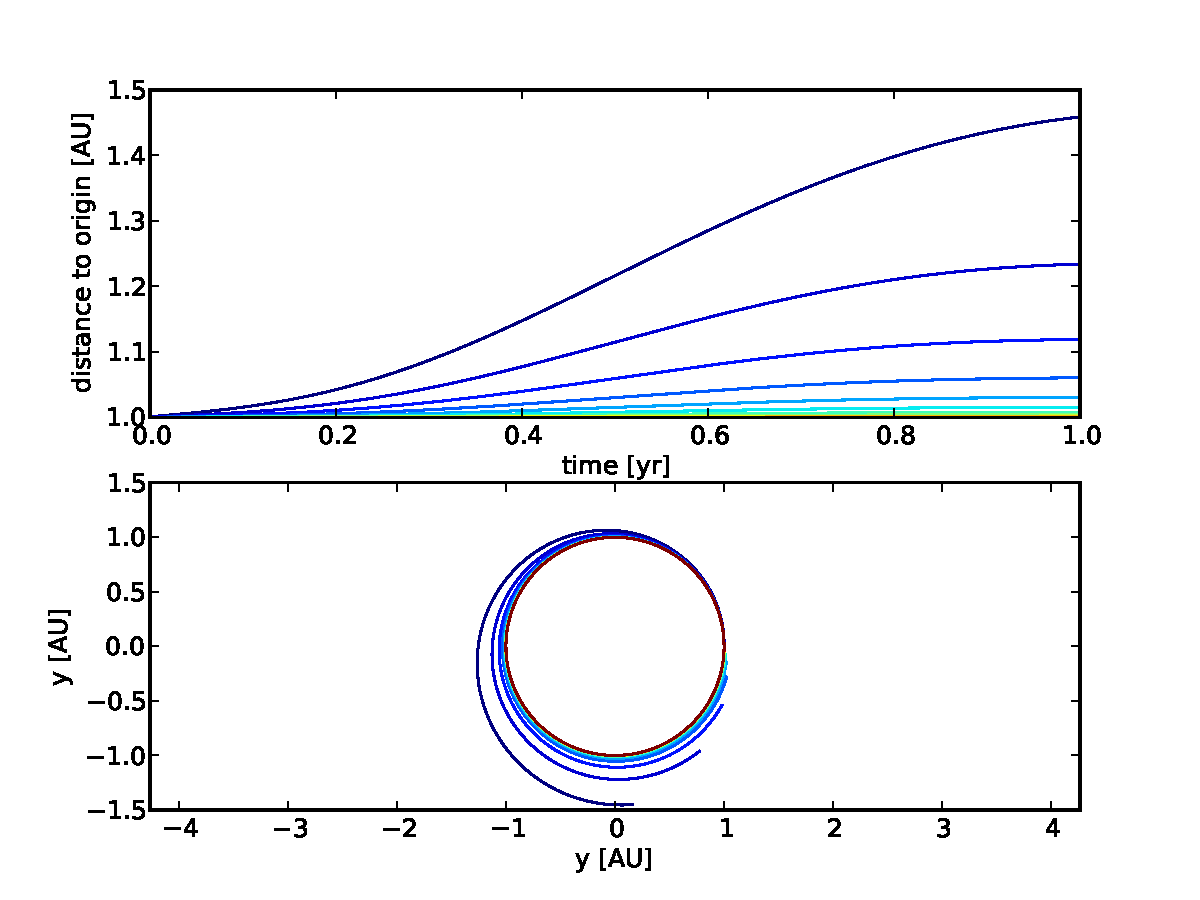
\includegraphics[width=1.0\linewidth]{../results/stability_orbits.pdf}
    \caption{Stability of the Earth's orbit with different time steps $\Delta t$. Bigger time steps give bigger deviance.}
    \label{fig:stab_euler}
\end{figure}

The orbits are calculated for the earth over the course of one year, with
the biggest time step resulting in a distance of almost $1.5AU$.

\subsubsection{Energy conservation}
By plotting the energies of the system, we expect the total energy to be
constant independently of how long we run the simulation.
\Cref{fig:energy_verlet} confirms this with the velocity verlet method,
showing the energies and the angular momentum of the Earth.
\Cref{fig:energy_euler} shows the corresponding calculation for the Forward
Euler method.

\begin{figure}[H]
    \centering
    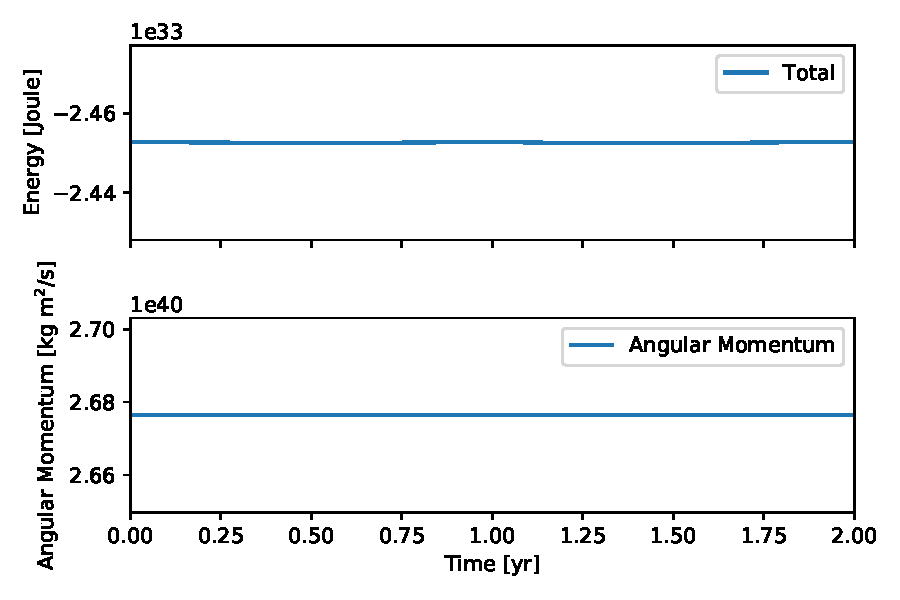
\includegraphics[width=0.8\linewidth]{energy_conservation_verlet.pdf}
    \caption{Conservation with the Verlet method. The energies and
        angular momentum of a two body system (the Earth and the Sun) in
        the reference frame of the largest object is plotted.}
    \label{fig:energy_verlet}
\end{figure}


\begin{figure}[H]
    \centering
    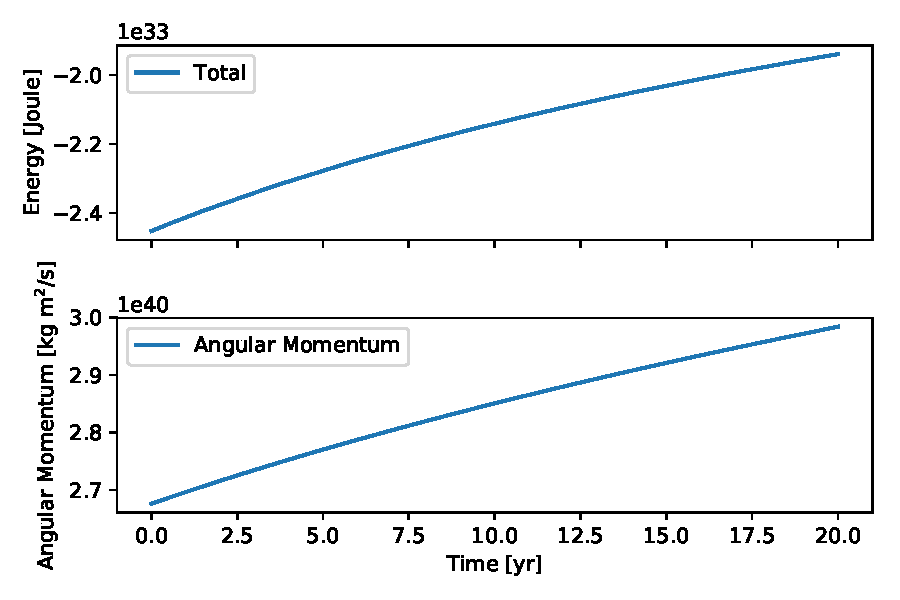
\includegraphics[width=0.8\linewidth]{energy_conservation_euler.pdf}
    \caption{Conservation with the Euler method. The energies and angular
        momentum of a two body system (the
    Earth and the Sun) in the reference frame of the largest object is
plotted.}
    \label{fig:energy_euler}
\end{figure}

\subsubsection{Escape velocity}
The following figure
shows how Earth leaves the orbit if the initial velocity is too large.
\begin{figure}[H]
    \centering
    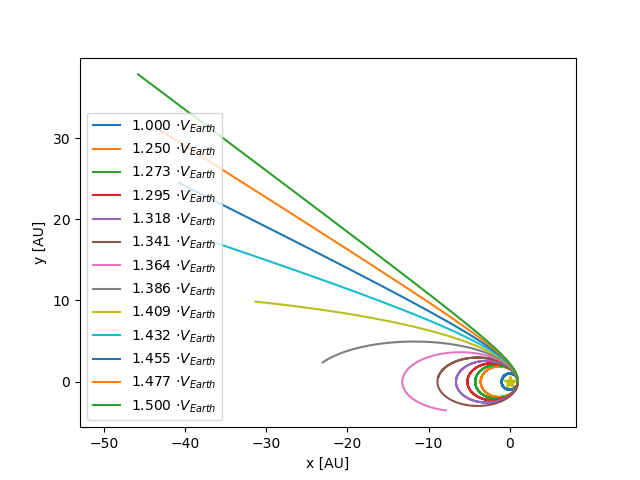
\includegraphics[width=1.0\linewidth]{../results/Esacpe_vel.png}
    \label{fig:name}
    \caption{The trajectory of Earth with different initial velocities compared to the real one}
\end{figure}
The analytical escape velocity is found with equation (10) and results in
\begin{equation}
    v_{e} = \sqrt{8\pi^2 AU^2/year^2} = \sqrt{2}2\pi AU/year \approx 1.414V_{Earth}\nonumber
\end{equation}


\subsection{Adding Jupiter}
\subsubsection{Normal Jupiter}
By adding Jupiter with the sun fixed in the centre 
\subsubsection{Massive Jupiter}
One we increase the mass of Jupiter to the mass of the sun, Earth
immediately loses its track and gets violently tossed between the two
objects (\cref{fig:jupiter1000x}). The energy is still conserved though,
as seen in \cref{fig:energyEarthJupiter}. Changing the time step to a
smaller one, we get the movement in \cref{fig:jupiter1000x2}, showing an
unstable system.

\begin{figure}[H]
    \centering
    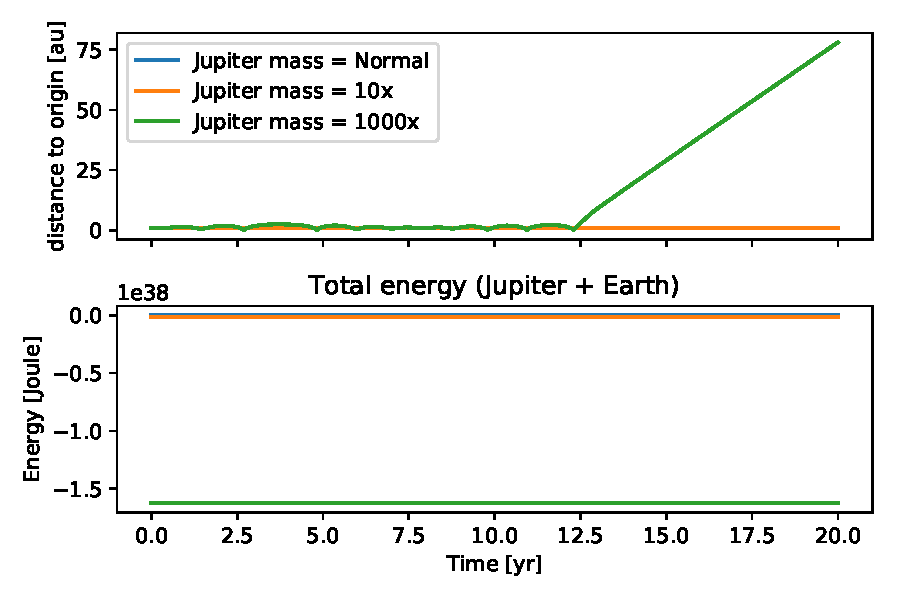
\includegraphics[width=0.8\linewidth]{energyEarthJupiter.pdf}
    \caption{Energy of earth while jupiter is present, different masses for
        the planet jupiter, with a fixed sun.  }
    \label{fig:energyEarthJupiter}
\end{figure}

\begin{figure}[H]
    \centering
    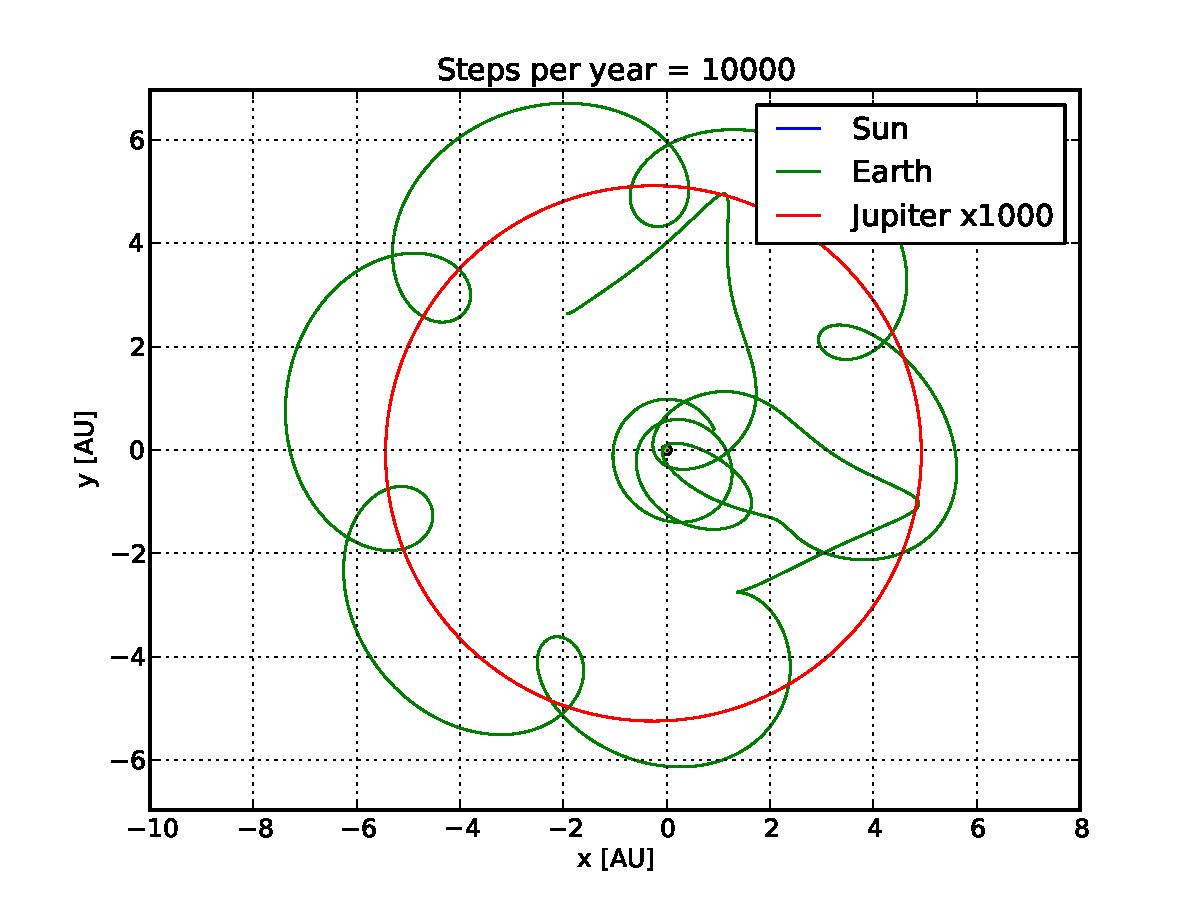
\includegraphics[width=1.0\linewidth]{../results/EJSx1000_1.pdf}
    \caption{The Earth-Jupiter-Sun system where the mass of jupiter is
    increased by a factor 1000, with the Sun held in position}
    \label{fig:jupiter1000x}
\end{figure}

\subsubsection{Three-body problem}
Letting the sun move as well, we get a plot similar to the one before in
\cref{fig:energyEarthJupiter2}. The corresponding orbits are shown in
\cref{fig:EJSx1000_moving}, showing a binary system with a planet getting
slung around.

\begin{figure}[htpb]
    \centering
    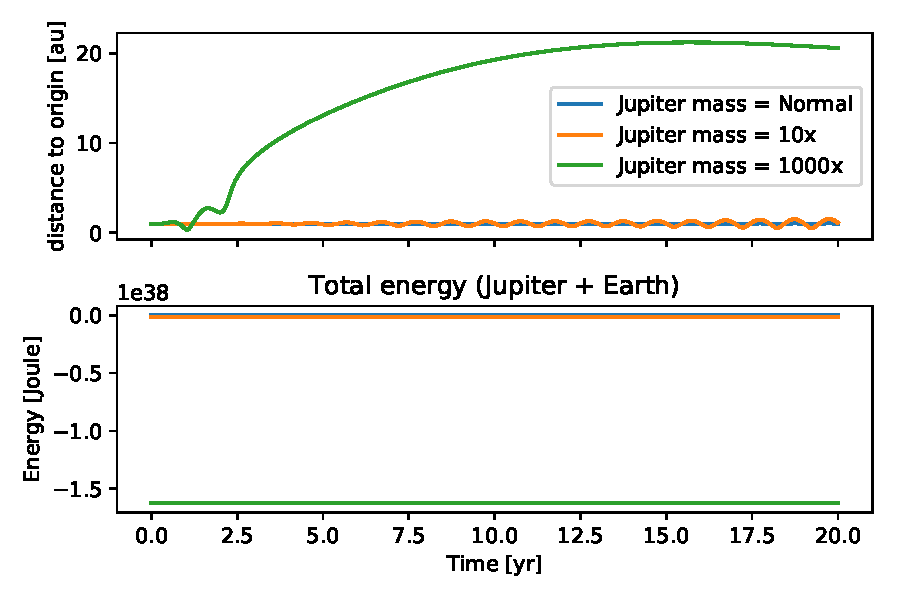
\includegraphics[width=0.8\linewidth]{energyEarthJupiter1.pdf}
    \caption{Energy of earth while jupiter is present, different masses for
        the planet jupiter, with a moving sun.  }
    \label{fig:energyEarthJupiter2}
\end{figure}

\begin{figure}[H]
    \centering
    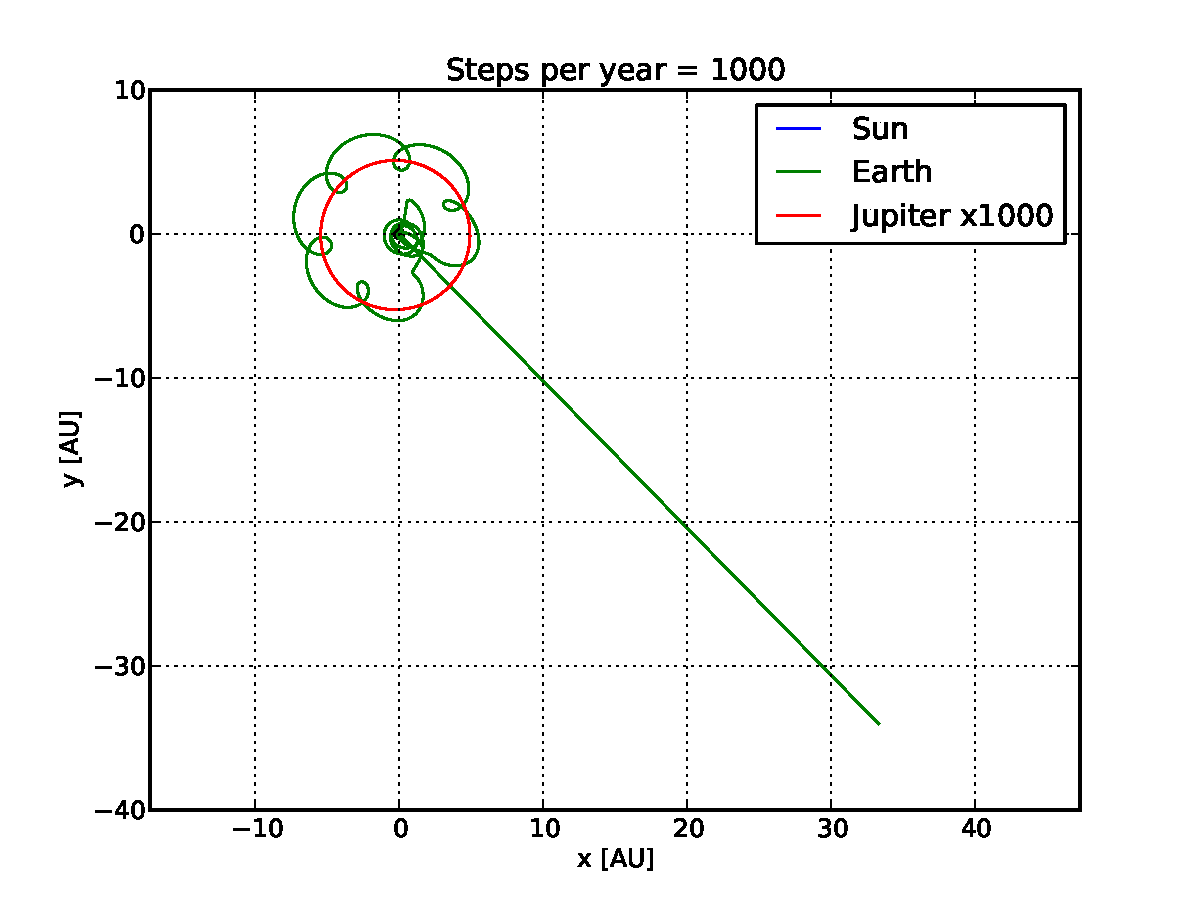
\includegraphics[width=1.0\linewidth]{../results/EJSx1000_2.pdf}
    \caption{The Earth-Jupiter-Sun system where the mass of jupiter is
    increased by a factor 1000, with the Sun held in position}
    \label{fig:jupiter1000x2}
\end{figure}

\begin{figure}[H]
    \centering
    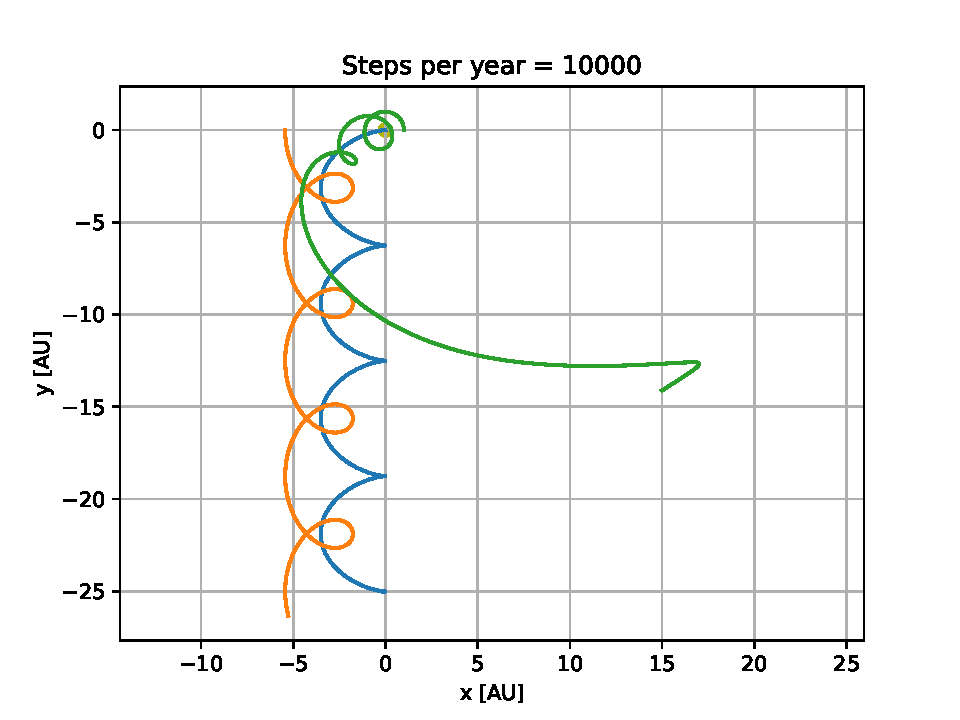
\includegraphics[width=1.0\linewidth]{../results/EJSx1000_moving.pdf}
    \caption{The Earth-Jupiter-Sun system where the mass of jupiter is
    increased by a factor 1000, with a moving Sun.}
    \label{fig:jupiter1000x2}
\end{figure}

\subsection{N-body problem}
With all the planets inserted, our solar looks satisfyingly familiar

\begin{figure}[H]
    \centering
    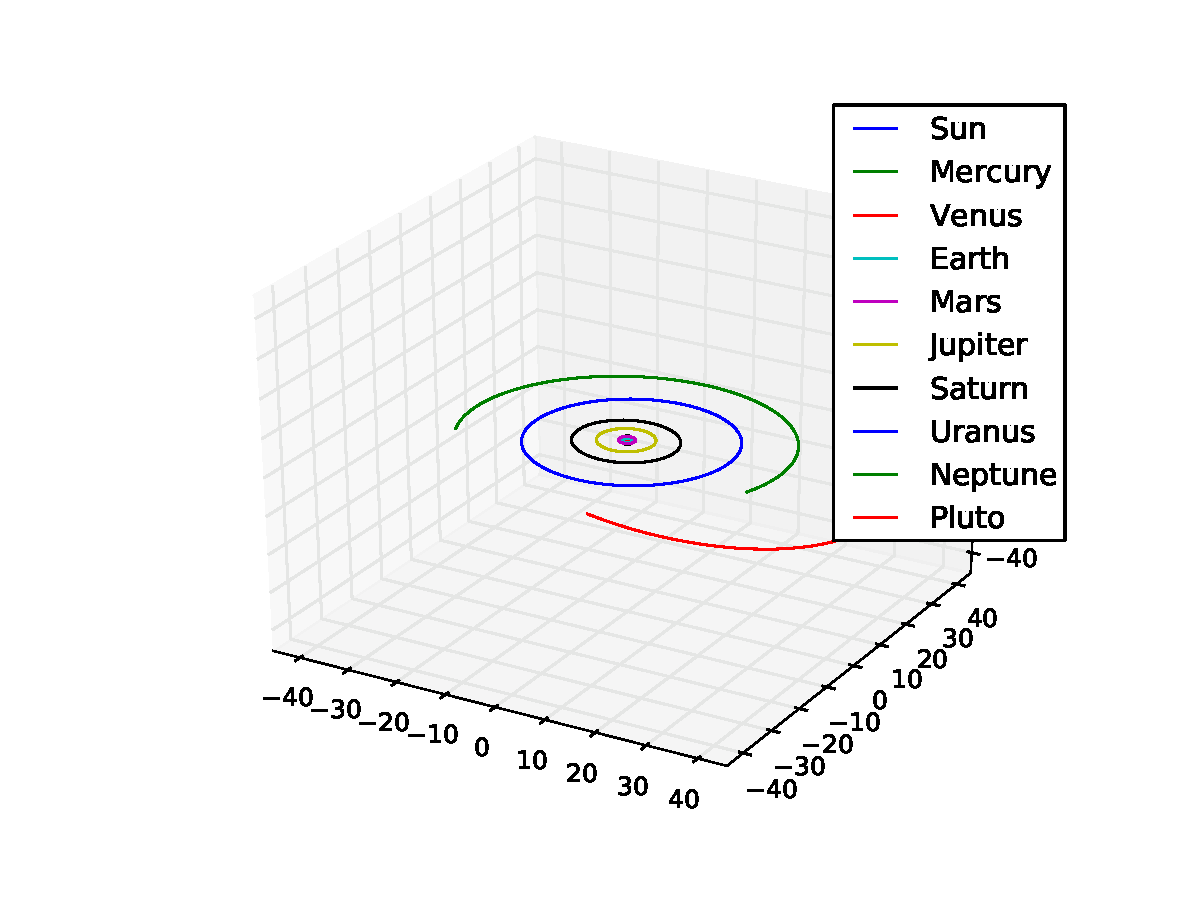
\includegraphics[width=1.0\linewidth]{../results/full_system.pdf}
    \label{fig:name}
    \caption{All ten objects of our solar system in three dimensions.}
\end{figure}

Zooming in, we can confirm that the inner planets also follow cyclical
orbits


\begin{figure}[H]
    \centering
    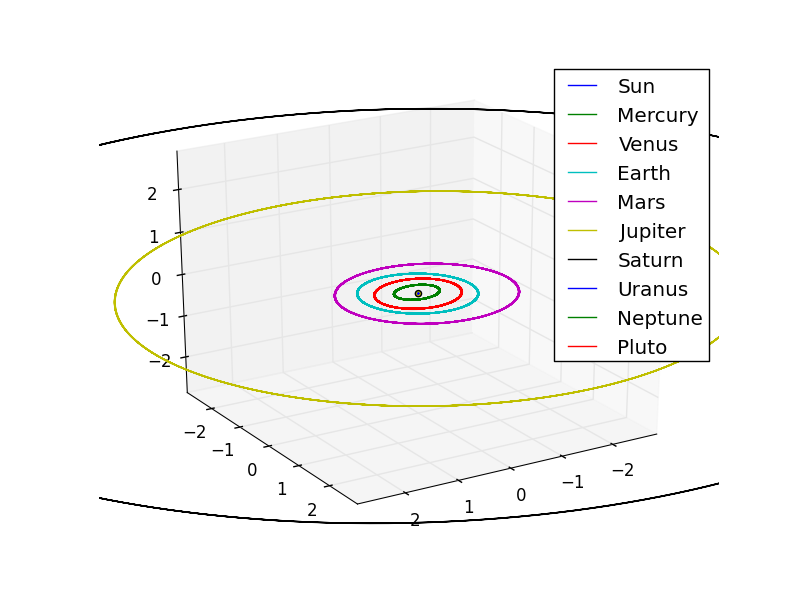
\includegraphics[width=1.0\linewidth]{../results/full_system_inner.png}
    \label{fig:name}
\end{figure}





\subsection{Mercury}
With the relativistic effects applied to Mercury, we observe how the
elliptical orbit slightly rotates around its elliptical orbit. The orbit
precesses 44.5 arcseconds in 100 years, which isnt very far from the
expected result of around 43 arcseconds.

\begin{figure}[H]
    \centering
    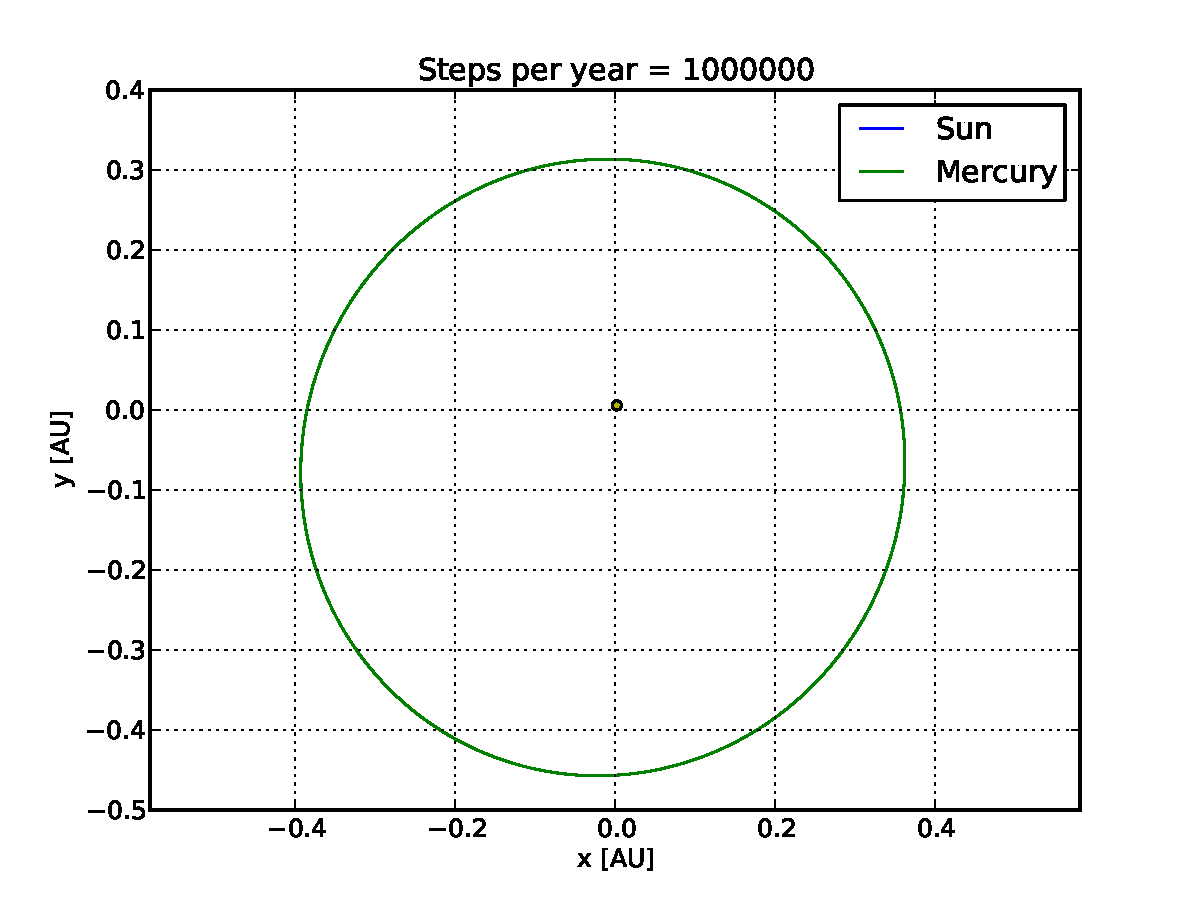
\includegraphics[width=1.0\linewidth]{../results/MercuryOrbit.pdf}
    \label{fig:name}
\end{figure}

The change is too small to recognized on the orbit, but by calculation, we
can find. As we can see on the following plot, the angle of its orbit
changes linearly.

\begin{figure}[H]
    \centering
    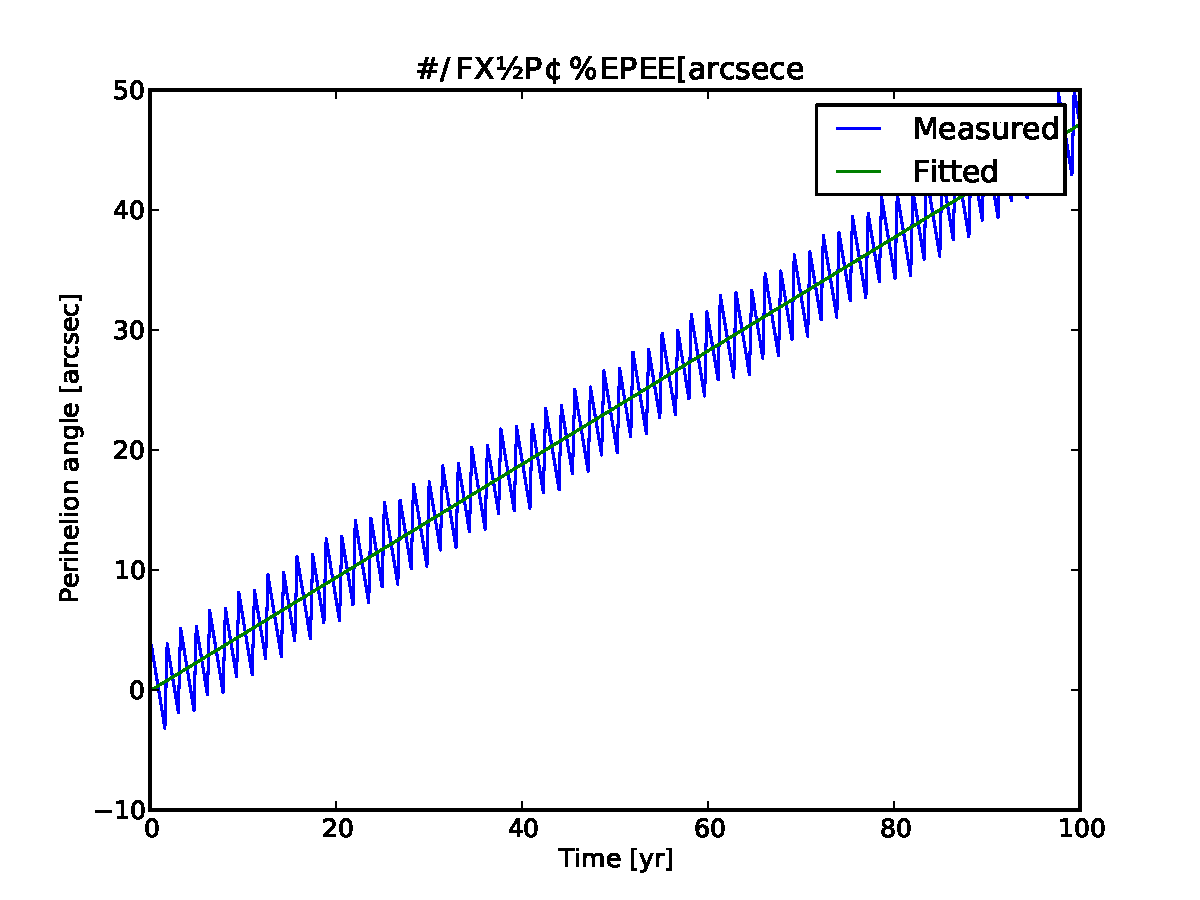
\includegraphics[width=1.0\linewidth]{../results/peri_precession}
    \label{fig:name}
\end{figure}


%%%%%%%%%%%%%%%%%%%%%%%%%%%%%%%%%%%%%%%%%%%%%%%%%%%%%%%%%%%%%%%%%%%%%%%%%%%
\section{Discussion and conclusions}

%%% COMPARE MERCURY PRECESSION TO KNOWN VALUE

\subsection{Comparison of methods}
As we predicted, the Verlet method produces far more precise results than Euler. With the Verlet method we were able to calculate the case of Mercury with $10^8$ time steps in 173.48 seconds. The program crashes due to overflow if it's run with Euler's method.
\subsection{Testing of $\Delta t$}
As seen in figure \cref{}, with sufficiently small time steps, the orbit
of the planet is stable. It slightly oscillates around $1AU$, which checks
out with the eccentricity of the earth being $0.0167$.

\subsection{Two-body system}
\subsubsection{Escape velocity}
As figure --- shows, the planet will remain in orbit for all initial velocities less than some value $v_e \in [1.409,1.432]v_{Earth}$. This checks out with the analytical value we calculated to be $v_e = 1.414\cdot v_{Earth}$.

\subsection{Three-body system}
\subsubsection{Massive Jupiter}
As we increased the mass of Jupiter, the Earth loses it's circular orbit as it starts getting pulled in different directions by the two massive objects. This is as expected as we have increased its mass to that of the sun, effectively making it a binary star system, except for the fact that the sun is fixed in the origin. 


\subsection{N-body system}
With all the initial conditions collected from NASA, our solar system takes form. As we have have modelled our system in all three dimensions, it appears that not all planets move in the same plane. And sure enough, Pluto's $17^O$ inclination reveals itself.





\section*{Appendix}
See https://github.com/halvarsu/FYS3150/ for code.

From \cite{lectureNotes}:

\begin{table}[H]
    \caption{Masses of the bodies in the solar system}
    \centering
    \begin{tabular}{| c | c | c | }
        \hline
        Body & Mass $\SI{10e24}{kg}$ & Distance to sun in AU\\
        \hline
        Sun      $\Sun$   & \SI{1.989e6}{}&  0 \\
        Mercury  $\Mercury$ & 0.3301    &  0.39 \\
        Venus    $\Venus$   & 4.867     &  0.72 \\
        Earth    $\Earth$   & 5.972     &  1 \\
        Moon     $\Moon$    & 0.073     &  1 \\
        Mars     $\Mars$    & 0.642     &  1.52 \\
        Jupiter  $\Jupiter$ & 1898      &  5.3 \\
        Saturn   $\Saturn$  & 568       &  9.54 \\
        Uranus   $\Uranus$  & 86.8      & 19.19 \\
        Neptune  $\Neptune$ & 102       & 30.06 \\
        Pluto    $\Pluto$   & 0.0146    & 39.53 \\
        \hline
    \end{tabular}
    \label{tab:CelestialMasses}
\end{table}


\bibliography{bib1}{}
\bibliographystyle{plain}

\end{multicols}


\end{document}
